


% Header, overrides base

    % Make sure that the sphinx doc style knows who it inherits from.
    \def\sphinxdocclass{article}

    % Declare the document class
    \documentclass[letterpaper,10pt,english]{/Library/Python/2.7/site-packages/Sphinx-1.2-py2.7.egg/sphinx/texinputs/sphinxhowto}

    % Imports
    \usepackage[utf8]{inputenc}
    \DeclareUnicodeCharacter{00A0}{\\nobreakspace}
    \usepackage[T1]{fontenc}
    \usepackage{babel}
    \usepackage{times}
    \usepackage{import}
    \usepackage[Bjarne]{/Library/Python/2.7/site-packages/Sphinx-1.2-py2.7.egg/sphinx/texinputs/fncychap}
    \usepackage{longtable}
    \usepackage{/Library/Python/2.7/site-packages/Sphinx-1.2-py2.7.egg/sphinx/texinputs/sphinx}
    \usepackage{multirow}

    \usepackage{amsmath}
    \usepackage{amssymb}
    \usepackage{ucs}
    \usepackage{enumerate}

    % Used to make the Input/Output rules follow around the contents.
    \usepackage{needspace}

    % Pygments requirements
    \usepackage{fancyvrb}
    \usepackage{color}
    % ansi colors additions
    \definecolor{darkgreen}{rgb}{.12,.54,.11}
    \definecolor{lightgray}{gray}{.95}
    \definecolor{brown}{rgb}{0.54,0.27,0.07}
    \definecolor{purple}{rgb}{0.5,0.0,0.5}
    \definecolor{darkgray}{gray}{0.25}
    \definecolor{lightred}{rgb}{1.0,0.39,0.28}
    \definecolor{lightgreen}{rgb}{0.48,0.99,0.0}
    \definecolor{lightblue}{rgb}{0.53,0.81,0.92}
    \definecolor{lightpurple}{rgb}{0.87,0.63,0.87}
    \definecolor{lightcyan}{rgb}{0.5,1.0,0.83}

    % Needed to box output/input
    \usepackage{tikz}
        \usetikzlibrary{calc,arrows,shadows}
    \usepackage[framemethod=tikz]{mdframed}

    \usepackage{alltt}

    % Used to load and display graphics
    \usepackage{graphicx}
    \graphicspath{ {figs/} }
    \usepackage[Export]{adjustbox} % To resize

    % used so that images for notebooks which have spaces in the name can still be included
    \usepackage{grffile}


    % For formatting output while also word wrapping.
    \usepackage{listings}
    \lstset{breaklines=true}
    \lstset{basicstyle=\small\ttfamily}
    \def\smaller{\fontsize{9.5pt}{9.5pt}\selectfont}

    %Pygments definitions
    
\makeatletter
\def\PY@reset{\let\PY@it=\relax \let\PY@bf=\relax%
    \let\PY@ul=\relax \let\PY@tc=\relax%
    \let\PY@bc=\relax \let\PY@ff=\relax}
\def\PY@tok#1{\csname PY@tok@#1\endcsname}
\def\PY@toks#1+{\ifx\relax#1\empty\else%
    \PY@tok{#1}\expandafter\PY@toks\fi}
\def\PY@do#1{\PY@bc{\PY@tc{\PY@ul{%
    \PY@it{\PY@bf{\PY@ff{#1}}}}}}}
\def\PY#1#2{\PY@reset\PY@toks#1+\relax+\PY@do{#2}}

\expandafter\def\csname PY@tok@gd\endcsname{\def\PY@tc##1{\textcolor[rgb]{0.63,0.00,0.00}{##1}}}
\expandafter\def\csname PY@tok@gu\endcsname{\let\PY@bf=\textbf\def\PY@tc##1{\textcolor[rgb]{0.50,0.00,0.50}{##1}}}
\expandafter\def\csname PY@tok@gt\endcsname{\def\PY@tc##1{\textcolor[rgb]{0.00,0.27,0.87}{##1}}}
\expandafter\def\csname PY@tok@gs\endcsname{\let\PY@bf=\textbf}
\expandafter\def\csname PY@tok@gr\endcsname{\def\PY@tc##1{\textcolor[rgb]{1.00,0.00,0.00}{##1}}}
\expandafter\def\csname PY@tok@cm\endcsname{\let\PY@it=\textit\def\PY@tc##1{\textcolor[rgb]{0.25,0.50,0.50}{##1}}}
\expandafter\def\csname PY@tok@vg\endcsname{\def\PY@tc##1{\textcolor[rgb]{0.10,0.09,0.49}{##1}}}
\expandafter\def\csname PY@tok@m\endcsname{\def\PY@tc##1{\textcolor[rgb]{0.40,0.40,0.40}{##1}}}
\expandafter\def\csname PY@tok@mh\endcsname{\def\PY@tc##1{\textcolor[rgb]{0.40,0.40,0.40}{##1}}}
\expandafter\def\csname PY@tok@go\endcsname{\def\PY@tc##1{\textcolor[rgb]{0.53,0.53,0.53}{##1}}}
\expandafter\def\csname PY@tok@ge\endcsname{\let\PY@it=\textit}
\expandafter\def\csname PY@tok@vc\endcsname{\def\PY@tc##1{\textcolor[rgb]{0.10,0.09,0.49}{##1}}}
\expandafter\def\csname PY@tok@il\endcsname{\def\PY@tc##1{\textcolor[rgb]{0.40,0.40,0.40}{##1}}}
\expandafter\def\csname PY@tok@cs\endcsname{\let\PY@it=\textit\def\PY@tc##1{\textcolor[rgb]{0.25,0.50,0.50}{##1}}}
\expandafter\def\csname PY@tok@cp\endcsname{\def\PY@tc##1{\textcolor[rgb]{0.74,0.48,0.00}{##1}}}
\expandafter\def\csname PY@tok@gi\endcsname{\def\PY@tc##1{\textcolor[rgb]{0.00,0.63,0.00}{##1}}}
\expandafter\def\csname PY@tok@gh\endcsname{\let\PY@bf=\textbf\def\PY@tc##1{\textcolor[rgb]{0.00,0.00,0.50}{##1}}}
\expandafter\def\csname PY@tok@ni\endcsname{\let\PY@bf=\textbf\def\PY@tc##1{\textcolor[rgb]{0.60,0.60,0.60}{##1}}}
\expandafter\def\csname PY@tok@nl\endcsname{\def\PY@tc##1{\textcolor[rgb]{0.63,0.63,0.00}{##1}}}
\expandafter\def\csname PY@tok@nn\endcsname{\let\PY@bf=\textbf\def\PY@tc##1{\textcolor[rgb]{0.00,0.00,1.00}{##1}}}
\expandafter\def\csname PY@tok@no\endcsname{\def\PY@tc##1{\textcolor[rgb]{0.53,0.00,0.00}{##1}}}
\expandafter\def\csname PY@tok@na\endcsname{\def\PY@tc##1{\textcolor[rgb]{0.49,0.56,0.16}{##1}}}
\expandafter\def\csname PY@tok@nb\endcsname{\def\PY@tc##1{\textcolor[rgb]{0.00,0.50,0.00}{##1}}}
\expandafter\def\csname PY@tok@nc\endcsname{\let\PY@bf=\textbf\def\PY@tc##1{\textcolor[rgb]{0.00,0.00,1.00}{##1}}}
\expandafter\def\csname PY@tok@nd\endcsname{\def\PY@tc##1{\textcolor[rgb]{0.67,0.13,1.00}{##1}}}
\expandafter\def\csname PY@tok@ne\endcsname{\let\PY@bf=\textbf\def\PY@tc##1{\textcolor[rgb]{0.82,0.25,0.23}{##1}}}
\expandafter\def\csname PY@tok@nf\endcsname{\def\PY@tc##1{\textcolor[rgb]{0.00,0.00,1.00}{##1}}}
\expandafter\def\csname PY@tok@si\endcsname{\let\PY@bf=\textbf\def\PY@tc##1{\textcolor[rgb]{0.73,0.40,0.53}{##1}}}
\expandafter\def\csname PY@tok@s2\endcsname{\def\PY@tc##1{\textcolor[rgb]{0.73,0.13,0.13}{##1}}}
\expandafter\def\csname PY@tok@vi\endcsname{\def\PY@tc##1{\textcolor[rgb]{0.10,0.09,0.49}{##1}}}
\expandafter\def\csname PY@tok@nt\endcsname{\let\PY@bf=\textbf\def\PY@tc##1{\textcolor[rgb]{0.00,0.50,0.00}{##1}}}
\expandafter\def\csname PY@tok@nv\endcsname{\def\PY@tc##1{\textcolor[rgb]{0.10,0.09,0.49}{##1}}}
\expandafter\def\csname PY@tok@s1\endcsname{\def\PY@tc##1{\textcolor[rgb]{0.73,0.13,0.13}{##1}}}
\expandafter\def\csname PY@tok@sh\endcsname{\def\PY@tc##1{\textcolor[rgb]{0.73,0.13,0.13}{##1}}}
\expandafter\def\csname PY@tok@sc\endcsname{\def\PY@tc##1{\textcolor[rgb]{0.73,0.13,0.13}{##1}}}
\expandafter\def\csname PY@tok@sx\endcsname{\def\PY@tc##1{\textcolor[rgb]{0.00,0.50,0.00}{##1}}}
\expandafter\def\csname PY@tok@bp\endcsname{\def\PY@tc##1{\textcolor[rgb]{0.00,0.50,0.00}{##1}}}
\expandafter\def\csname PY@tok@c1\endcsname{\let\PY@it=\textit\def\PY@tc##1{\textcolor[rgb]{0.25,0.50,0.50}{##1}}}
\expandafter\def\csname PY@tok@kc\endcsname{\let\PY@bf=\textbf\def\PY@tc##1{\textcolor[rgb]{0.00,0.50,0.00}{##1}}}
\expandafter\def\csname PY@tok@c\endcsname{\let\PY@it=\textit\def\PY@tc##1{\textcolor[rgb]{0.25,0.50,0.50}{##1}}}
\expandafter\def\csname PY@tok@mf\endcsname{\def\PY@tc##1{\textcolor[rgb]{0.40,0.40,0.40}{##1}}}
\expandafter\def\csname PY@tok@err\endcsname{\def\PY@bc##1{\setlength{\fboxsep}{0pt}\fcolorbox[rgb]{1.00,0.00,0.00}{1,1,1}{\strut ##1}}}
\expandafter\def\csname PY@tok@kd\endcsname{\let\PY@bf=\textbf\def\PY@tc##1{\textcolor[rgb]{0.00,0.50,0.00}{##1}}}
\expandafter\def\csname PY@tok@ss\endcsname{\def\PY@tc##1{\textcolor[rgb]{0.10,0.09,0.49}{##1}}}
\expandafter\def\csname PY@tok@sr\endcsname{\def\PY@tc##1{\textcolor[rgb]{0.73,0.40,0.53}{##1}}}
\expandafter\def\csname PY@tok@mo\endcsname{\def\PY@tc##1{\textcolor[rgb]{0.40,0.40,0.40}{##1}}}
\expandafter\def\csname PY@tok@kn\endcsname{\let\PY@bf=\textbf\def\PY@tc##1{\textcolor[rgb]{0.00,0.50,0.00}{##1}}}
\expandafter\def\csname PY@tok@mi\endcsname{\def\PY@tc##1{\textcolor[rgb]{0.40,0.40,0.40}{##1}}}
\expandafter\def\csname PY@tok@gp\endcsname{\let\PY@bf=\textbf\def\PY@tc##1{\textcolor[rgb]{0.00,0.00,0.50}{##1}}}
\expandafter\def\csname PY@tok@o\endcsname{\def\PY@tc##1{\textcolor[rgb]{0.40,0.40,0.40}{##1}}}
\expandafter\def\csname PY@tok@kr\endcsname{\let\PY@bf=\textbf\def\PY@tc##1{\textcolor[rgb]{0.00,0.50,0.00}{##1}}}
\expandafter\def\csname PY@tok@s\endcsname{\def\PY@tc##1{\textcolor[rgb]{0.73,0.13,0.13}{##1}}}
\expandafter\def\csname PY@tok@kp\endcsname{\def\PY@tc##1{\textcolor[rgb]{0.00,0.50,0.00}{##1}}}
\expandafter\def\csname PY@tok@w\endcsname{\def\PY@tc##1{\textcolor[rgb]{0.73,0.73,0.73}{##1}}}
\expandafter\def\csname PY@tok@kt\endcsname{\def\PY@tc##1{\textcolor[rgb]{0.69,0.00,0.25}{##1}}}
\expandafter\def\csname PY@tok@ow\endcsname{\let\PY@bf=\textbf\def\PY@tc##1{\textcolor[rgb]{0.67,0.13,1.00}{##1}}}
\expandafter\def\csname PY@tok@sb\endcsname{\def\PY@tc##1{\textcolor[rgb]{0.73,0.13,0.13}{##1}}}
\expandafter\def\csname PY@tok@k\endcsname{\let\PY@bf=\textbf\def\PY@tc##1{\textcolor[rgb]{0.00,0.50,0.00}{##1}}}
\expandafter\def\csname PY@tok@se\endcsname{\let\PY@bf=\textbf\def\PY@tc##1{\textcolor[rgb]{0.73,0.40,0.13}{##1}}}
\expandafter\def\csname PY@tok@sd\endcsname{\let\PY@it=\textit\def\PY@tc##1{\textcolor[rgb]{0.73,0.13,0.13}{##1}}}

\def\PYZbs{\char`\\}
\def\PYZus{\char`\_}
\def\PYZob{\char`\{}
\def\PYZcb{\char`\}}
\def\PYZca{\char`\^}
\def\PYZam{\char`\&}
\def\PYZlt{\char`\<}
\def\PYZgt{\char`\>}
\def\PYZsh{\char`\#}
\def\PYZpc{\char`\%}
\def\PYZdl{\char`\$}
\def\PYZhy{\char`\-}
\def\PYZsq{\char`\'}
\def\PYZdq{\char`\"}
\def\PYZti{\char`\~}
% for compatibility with earlier versions
\def\PYZat{@}
\def\PYZlb{[}
\def\PYZrb{]}
\makeatother


    %Set pygments styles if needed...
    
        \definecolor{nbframe-border}{rgb}{0.867,0.867,0.867}
        \definecolor{nbframe-bg}{rgb}{0.969,0.969,0.969}
        \definecolor{nbframe-in-prompt}{rgb}{0.0,0.0,0.502}
        \definecolor{nbframe-out-prompt}{rgb}{0.545,0.0,0.0}

        \newenvironment{ColorVerbatim}
        {\begin{mdframed}[%
            roundcorner=1.0pt, %
            backgroundcolor=nbframe-bg, %
            userdefinedwidth=1\linewidth, %
            leftmargin=0.1\linewidth, %
            innerleftmargin=0pt, %
            innerrightmargin=0pt, %
            linecolor=nbframe-border, %
            linewidth=1pt, %
            usetwoside=false, %
            everyline=true, %
            innerlinewidth=3pt, %
            innerlinecolor=nbframe-bg, %
            middlelinewidth=1pt, %
            middlelinecolor=nbframe-bg, %
            outerlinewidth=0.5pt, %
            outerlinecolor=nbframe-border, %
            needspace=0pt
        ]}
        {\end{mdframed}}
        
        \newenvironment{InvisibleVerbatim}
        {\begin{mdframed}[leftmargin=0.1\linewidth,innerleftmargin=3pt,innerrightmargin=3pt, userdefinedwidth=1\linewidth, linewidth=0pt, linecolor=white, usetwoside=false]}
        {\end{mdframed}}

        \renewenvironment{Verbatim}[1][\unskip]
        {\begin{alltt}\smaller}
        {\end{alltt}}
    

    % Help prevent overflowing lines due to urls and other hard-to-break 
    % entities.  This doesn't catch everything...
    \sloppy

    % Document level variables
    \title{HW01}
    \date{January 26, 2014}
    \release{}
    \author{Andy Reagan}
    \renewcommand{\releasename}{}

    % TODO: Add option for the user to specify a logo for his/her export.
    \newcommand{\sphinxlogo}{}

    % Make the index page of the document.
    \makeindex

    % Import sphinx document type specifics.
     


% Body

    % Start of the document
    \begin{document}

        
            \maketitle
        

        


        
\section{problem 1}Consider the IVP \[ y' = ay, y(x_0) = y_0,\] where $a$ is a constant.
Following the lines of derivation of the global error, find how the sign
of the global error depends on $y_0$ and $a$.\subsection{solution}from equation 1.4 in the notes, we have the following expression for the
global error:
\[ \epsilon _{i+1} = \epsilon _i + h(f(x_i,y_i)-f(x_i,Y_i))+\frac{h^2}{2} y''(x^*_i ) .\]
for our equation, we have $y(x) = y_0 e^{a(x-x_0)}$ and equation 1.4
becomes
\[ \epsilon_{i+1} = \epsilon_i + ha(y_i - Y_i) + \frac{h^2}{2} a^2 y_0 e^{a(x_i^*-x_0)} .\]
noticing that by defition, $\epsilon _i = y_i - Y_i$, we can rewrite the
above as
\[ \epsilon_{i+1} = (1+ah) \epsilon_i + \frac{h^2}{2} a^2 y_0 e^{a(x_i^*-x_0)} .\]
leaving out the terms that are always positive, we then have (assuming
$1+ah>0$, and denoting sgn the sign function)
\[ sgn(\epsilon_{i+1}) = sgn(\epsilon_i + y_0) .\] now since
$\epsilon _0$ is the local error (the last term in 1.4), the above has
shown that the sign of $\epsilon _0$ is the same as the sign of $y_0$.
therefore, the sign of the global error follows the sign of $y_0$.

    % Make sure that atleast 4 lines are below the HR
    \needspace{4\baselineskip}

    
        \vspace{6pt}
        \makebox[0.1\linewidth]{\smaller\hfill\tt\color{nbframe-in-prompt}In\hspace{4pt}{[}2{]}:\hspace{4pt}}\\*
        \vspace{-2.65\baselineskip}
        \begin{ColorVerbatim}
            \vspace{-0.7\baselineskip}
            \begin{Verbatim}[commandchars=\\\{\}]
\PY{k+kn}{from} \PY{n+nn}{numpy} \PY{k+kn}{import} \PY{o}{*}

\PY{k}{def} \PY{n+nf}{sign}\PY{p}{(}\PY{n}{x}\PY{p}{)}\PY{p}{:}
    \PY{k}{if} \PY{n}{x}\PY{o}{\PYZlt{}}\PY{l+m+mi}{0}\PY{p}{:}
        \PY{k}{return} \PY{l+s}{\PYZsq{}}\PY{l+s}{negative}\PY{l+s}{\PYZsq{}}
    \PY{k}{else}\PY{p}{:}
        \PY{k}{return} \PY{l+s}{\PYZsq{}}\PY{l+s}{positive}\PY{l+s}{\PYZsq{}}

\PY{n}{h} \PY{o}{=} \PY{l+m+mf}{0.1}
\PY{n}{x} \PY{o}{=} \PY{n}{linspace}\PY{p}{(}\PY{l+m+mi}{0}\PY{p}{,}\PY{l+m+mi}{1}\PY{p}{,}\PY{n}{num}\PY{o}{=}\PY{n+nb}{int}\PY{p}{(}\PY{l+m+mi}{1}\PY{o}{/}\PY{n}{h}\PY{o}{+}\PY{l+m+mi}{1}\PY{p}{)}\PY{p}{)}

\PY{k}{for} \PY{n}{a} \PY{o+ow}{in} \PY{p}{[}\PY{l+m+mi}{1}\PY{p}{,}\PY{o}{\PYZhy{}}\PY{l+m+mi}{1}\PY{p}{]}\PY{p}{:}
    \PY{k}{for} \PY{n}{y0} \PY{o+ow}{in} \PY{p}{[}\PY{l+m+mi}{1}\PY{p}{,}\PY{o}{\PYZhy{}}\PY{l+m+mi}{1}\PY{p}{]}\PY{p}{:}
        \PY{n}{y} \PY{o}{=} \PY{n}{y0}
        \PY{k}{for} \PY{n}{i} \PY{o+ow}{in} \PY{n+nb}{xrange}\PY{p}{(}\PY{l+m+mi}{10}\PY{p}{)}\PY{p}{:}
            \PY{n}{y} \PY{o}{+}\PY{o}{=} \PY{n}{h}\PY{o}{*}\PY{n}{a}\PY{o}{*}\PY{n}{y}
        
        \PY{k}{print} \PY{l+s}{\PYZsq{}}\PY{l+s}{for y0=\PYZob{}0\PYZcb{},a=\PYZob{}1\PYZcb{}, the sign of global error is \PYZob{}2\PYZcb{}}\PY{l+s}{\PYZsq{}}\PY{o}{.}\PY{n}{format}\PY{p}{(}\PY{n}{y0}\PY{p}{,}\PY{n}{a}\PY{p}{,}\PY{n}{sign}\PY{p}{(}\PY{n}{y}\PY{p}{)}\PY{p}{)}
\end{Verbatim}

            
                \vspace{-0.2\baselineskip}
            
        \end{ColorVerbatim}
    

    

        % If the first block is an image, minipage the image.  Else
        % request a certain amount of space for the input text.
        \needspace{4\baselineskip}
        
        

            % Add document contents.
            
                \begin{InvisibleVerbatim}
                \vspace{-0.5\baselineskip}
\begin{alltt}for y0=1,a=1, the sign of global error is positive
for y0=-1,a=1, the sign of global error is negative
for y0=1,a=-1, the sign of global error is positive
for y0=-1,a=-1, the sign of global error is negative
\end{alltt}

            \end{InvisibleVerbatim}
            
        
    
\section{problem 2}find the coefficient $B$ in the midpoint method (1.19)\subsection{solution}our scheme is written as

\[ Y_{i+1} = Y_i + hf(x_i +h/2, Y_i + Bh) .\]

to find $B$, we compare the taylor expansion of this scheme and the
analytical solution. the taylor series for the numerical scheme is thus
\[ Y_{i+1} = Y_i + hf(x_i,Y_i) + \frac{h^2}{2} f_x (x_i,Y_i) + Bh^2 f_y(x_i,Y_i) + O(h^3) .\]
from the notes, the taylor series for the analytical solution is
\[ y_{i+1} = y_i + hf(x_i,y_i) + \frac{h^2}{2} (f_x (x_i,Y_i) + f_y(x_i,Y_i)f(x_i,y_i)) + O(h^3) .\]
to compute the local error, assume that $y_i = Y_i$ and subtracting
these two equations above, we have
\[ \epsilon _{i+1}  = \frac{h^2}{2}f_y(x_i,Y_i)f(x_i,y_i) - Bh^2 f_y(x_i,Y_i) + O(h^3) .\]
setting $\epsilon _{i+1} = O(h^3)$ and solving for $B$ we have that
\[ B = f(x_i,y_i) / 2.\]\section{problem 3}Derive the expression for the local truncation error of the Midpoint
method.\subsection{solution}first, I adopt the notation used in the notes, and write the analytical
taylor series as
\[ y_{i+1} = y_i + hf + \frac{h^2}{2} (f_x +ff_y) + \frac{h^3}{6} (f_{xx} + f_x f_y + 2 f f_{xy} + f (f_y)^2 + f^2 f_{yy} ) + O(h^4) .\]
now for the midpoint method, we have
\[ Y_{i+1} = Y_i + hf + \frac{h^2}{2} (f_x +ff_y) + \frac{h^3}{8} (f_{xx} + 2 f f_{xy} +  f^2 f_{yy} ) + O(h^4) .\]
subtracting these two, the error is
\[ \epsilon _{i+1}  = h^3 \left [ \left (\frac{1}{6} - \frac{1}{8} \right )  \left ( f_{xx} + 2ff_{xy} + f^2 f_{yy} \right ) + \frac{1}{6} \left ( f_xf_y + f (f_y)^2 \right ) \right ] + O(h^4)\]
and simplifying, this is
\[ \epsilon _{i+1}  = h^3 \left [ \frac{1}{24}  \left ( f_{xx} + 2ff_{xy} + f^2 f_{yy} \right ) + \frac{1}{6} \left ( f_xf_y + f (f_y)^2 \right ) \right ] + O(h^4).\]\section{problem 4}Solve the IVP $y' = \sqrt{y}, y(0) = 1$ for $x\in [0,1]$ using three
methods: simple Euler, modified Euler, and Midpoint. In each case, use
two values for the step size: $h = 0.1$ and $h=0.05$. Make a table that
shows your numerical error. By what factor does the error decrease when
the step size decreases from 0.1 to 0.05?

Are you results consistent with the expressions for the the local
truncation errors of these three methods? Namely:

\begin{enumerate}
\def\labelenumi{\arabic{enumi}.}
\item
  Do the dependencies of theses errors on $h$ agree with the theoretical
  predictions?
\item
  Does the sign of the error from the simple Euler method agree with
  that which follows from the derivation in Section 1.3 for this
  specific $y(x)$?
\item
  Do the signs and relative magnitudes of the errors of the modified
  Euler and Midpoint methods agree with the result of Sec 1.6 and your
  result in problem 3?
\end{enumerate}\subsection{solution}

    % Make sure that atleast 4 lines are below the HR
    \needspace{4\baselineskip}

    
        \vspace{6pt}
        \makebox[0.1\linewidth]{\smaller\hfill\tt\color{nbframe-in-prompt}In\hspace{4pt}{[}11{]}:\hspace{4pt}}\\*
        \vspace{-2.65\baselineskip}
        \begin{ColorVerbatim}
            \vspace{-0.7\baselineskip}
            \begin{Verbatim}[commandchars=\\\{\}]
\PY{n}{truth} \PY{o}{=} \PY{p}{(}\PY{p}{(}\PY{l+m+mf}{1.0}\PY{o}{+}\PY{l+m+mf}{2.0}\PY{p}{)}\PY{o}{*}\PY{o}{*}\PY{l+m+mi}{2}\PY{p}{)}\PY{o}{/}\PY{l+m+mf}{4.0}

\PY{n}{y0} \PY{o}{=} \PY{l+m+mf}{1.0}

\PY{k}{print}
\PY{k}{print} \PY{l+s}{\PYZsq{}}\PY{l+s}{\PYZhy{}}\PY{l+s}{\PYZsq{}}\PY{o}{*}\PY{l+m+mi}{52}
\PY{k}{print} \PY{l+s}{\PYZsq{}}\PY{l+s}{     h         euler       mod euler     midpoint  }\PY{l+s+se}{\PYZbs{}n}\PY{l+s}{\PYZsq{}}
\PY{k}{print} \PY{l+s}{\PYZsq{}}\PY{l+s}{\PYZhy{}}\PY{l+s}{\PYZsq{}}\PY{o}{*}\PY{l+m+mi}{52}

\PY{c}{\PYZsh{} loop over step size}
\PY{k}{for} \PY{n}{h} \PY{o+ow}{in} \PY{p}{[}\PY{o}{.}\PY{l+m+mo}{05}\PY{p}{,}\PY{o}{.}\PY{l+m+mi}{1}\PY{p}{]}\PY{p}{:}
    \PY{n}{x} \PY{o}{=} \PY{n}{linspace}\PY{p}{(}\PY{l+m+mi}{0}\PY{p}{,}\PY{l+m+mi}{1}\PY{p}{,}\PY{n}{num}\PY{o}{=}\PY{n+nb}{int}\PY{p}{(}\PY{l+m+mi}{1}\PY{o}{/}\PY{n}{h}\PY{o}{+}\PY{l+m+mi}{1}\PY{p}{)}\PY{p}{)}

    \PY{k}{print} \PY{l+s}{\PYZsq{}}\PY{l+s}{\PYZob{}0:8.03f\PYZcb{} }\PY{l+s}{\PYZsq{}}\PY{o}{.}\PY{n}{format}\PY{p}{(}\PY{n}{h}\PY{p}{)}\PY{p}{,}
    
    \PY{c}{\PYZsh{} simple euler}
    \PY{n}{y} \PY{o}{=} \PY{n}{y0}
    \PY{k}{for} \PY{n}{i} \PY{o+ow}{in} \PY{n}{x}\PY{p}{[}\PY{l+m+mi}{1}\PY{p}{:}\PY{p}{]}\PY{p}{:}
        \PY{n}{y} \PY{o}{=} \PY{n}{y}\PY{o}{+}\PY{n}{h}\PY{o}{*}\PY{n}{sqrt}\PY{p}{(}\PY{n}{y}\PY{p}{)}

    \PY{k}{print}\PY{l+s}{\PYZsq{}}\PY{l+s}{  \PYZob{}0:8.03f\PYZcb{}   }\PY{l+s}{\PYZsq{}}\PY{o}{.}\PY{n}{format}\PY{p}{(}\PY{n}{truth}\PY{o}{\PYZhy{}}\PY{n}{y}\PY{p}{)}\PY{p}{,}
    
    \PY{c}{\PYZsh{} modified euler}
    \PY{n}{y} \PY{o}{=} \PY{n}{y0}
    \PY{k}{for} \PY{n}{i} \PY{o+ow}{in} \PY{n}{x}\PY{p}{[}\PY{l+m+mi}{1}\PY{p}{:}\PY{p}{]}\PY{p}{:}
        \PY{n}{k1} \PY{o}{=} \PY{n}{sqrt}\PY{p}{(}\PY{n}{y}\PY{p}{)}
        \PY{n}{k2} \PY{o}{=} \PY{n}{sqrt}\PY{p}{(}\PY{n}{y}\PY{o}{+}\PY{n}{h}\PY{o}{*}\PY{n}{k1}\PY{p}{)}
        \PY{n}{y} \PY{o}{=} \PY{n}{y} \PY{o}{+} \PY{l+m+mf}{0.5}\PY{o}{*}\PY{n}{h}\PY{o}{*}\PY{p}{(}\PY{n}{k1}\PY{o}{+}\PY{n}{k2}\PY{p}{)}
    \PY{k}{print} \PY{l+s}{\PYZsq{}}\PY{l+s}{   \PYZob{}0:8.05f\PYZcb{}  }\PY{l+s}{\PYZsq{}}\PY{o}{.}\PY{n}{format}\PY{p}{(}\PY{n}{truth}\PY{o}{\PYZhy{}}\PY{n}{y}\PY{p}{)}\PY{p}{,}
    
    \PY{c}{\PYZsh{} midpoint}
    \PY{n}{y} \PY{o}{=} \PY{n}{y0}
    \PY{k}{for} \PY{n}{i} \PY{o+ow}{in} \PY{n}{x}\PY{p}{[}\PY{l+m+mi}{1}\PY{p}{:}\PY{p}{]}\PY{p}{:}
        \PY{n}{k1} \PY{o}{=} \PY{n}{sqrt}\PY{p}{(}\PY{n}{y}\PY{p}{)}
        \PY{n}{k2} \PY{o}{=} \PY{n}{sqrt}\PY{p}{(}\PY{n}{y}\PY{o}{+}\PY{l+m+mf}{0.5}\PY{o}{*}\PY{n}{h}\PY{o}{*}\PY{n}{k1}\PY{p}{)}
        \PY{c}{\PYZsh{} sqrt(y+h*0.5*sqrt(y))}
        \PY{n}{y} \PY{o}{=} \PY{n}{y}\PY{o}{+}\PY{n}{h}\PY{o}{*}\PY{n}{k2}
    \PY{k}{print}\PY{l+s}{\PYZsq{}}\PY{l+s}{   \PYZob{}0:8.05f\PYZcb{}  }\PY{l+s+se}{\PYZbs{}n}\PY{l+s}{\PYZsq{}}\PY{o}{.}\PY{n}{format}\PY{p}{(}\PY{n}{truth}\PY{o}{\PYZhy{}}\PY{n}{y}\PY{p}{)}
    \PY{k}{print} \PY{l+s}{\PYZsq{}}\PY{l+s}{\PYZhy{}}\PY{l+s}{\PYZsq{}}\PY{o}{*}\PY{l+m+mi}{52}
\end{Verbatim}

            
                \vspace{-0.2\baselineskip}
            
        \end{ColorVerbatim}
    

    

        % If the first block is an image, minipage the image.  Else
        % request a certain amount of space for the input text.
        \needspace{4\baselineskip}
        
        

            % Add document contents.
            
                \begin{InvisibleVerbatim}
                \vspace{-0.5\baselineskip}
\begin{alltt}
----------------------------------------------------
     h         euler       mod euler     midpoint

----------------------------------------------------
   0.050       0.015        0.00015       0.00008

----------------------------------------------------
   0.100       0.030        0.00060       0.00031

----------------------------------------------------
\end{alltt}

            \end{InvisibleVerbatim}
            
        
    
The errors decrease linearly for the Euler method (a factor of 2) and by
a factor of 4 for the second-order methods. This is expected from the
accuracy of these schemes. The dependencies on $h$ do agree with the
theory.

The sign of the error for Simple Euler does agree with section 1.3,
since $y_0 > 0$ and $y'' > 0$ would predict an error $>$ 0. Indeed the
error is greater than 0.

Both errors are positive, and this partially agrees with prediction,
since $y_0 > 0$ and $y'' > 0$. The Midpoint method is approximately
twice as accurate here, and this relative magnitude of accurarcy
increase agrees. Our theory has the coefficient of -1/12 in the error of
the ME method, and the coefficient of 1/24 in the Midpoint method, so we
would expect this halving of the error seen here.

The term with leading 1/6 in both errors is 1/24 for this $y$, and the
other term remains with $-1/4 \cdot \sqrt{y}$. What does not agree is
the sign of the Midpoint error, which we would now expect to be
negative, but is positive here.\section{problem 5}A skydiver jumps into a fluid that is resistant with direct proportion
to his velocity $v$.\subsection{solution}Before his parachute opens to slow him, his velocity follows the ODE:
\[ \frac{dv}{dt} = g - \frac{k}{m} v .\] Setting the parameters such
that his maximum velocity reaches 80 m/s, we solve for $dv/dt = 0$ for
his asymptotical terminal velocity. This is solving
\[ 0 = 9.8 - 80 \frac{k}{m}.\] Since there are two unknowns, and one
equation, we do not consider mass. This results in $k$ equal to

    % Make sure that atleast 4 lines are below the HR
    \needspace{4\baselineskip}

    
        \vspace{6pt}
        \makebox[0.1\linewidth]{\smaller\hfill\tt\color{nbframe-in-prompt}In\hspace{4pt}{[}8{]}:\hspace{4pt}}\\*
        \vspace{-2.65\baselineskip}
        \begin{ColorVerbatim}
            \vspace{-0.7\baselineskip}
            \begin{Verbatim}[commandchars=\\\{\}]
\PY{n}{g} \PY{o}{=} \PY{l+m+mf}{9.8}
\PY{n}{k} \PY{o}{=} \PY{n}{g}\PY{o}{/}\PY{l+m+mf}{35.76} \PY{c}{\PYZsh{} that\PYZsq{}s 80mph in m/s}
\PY{k}{print} \PY{n}{k}
\end{Verbatim}

            
                \vspace{-0.2\baselineskip}
            
        \end{ColorVerbatim}
    

    

        % If the first block is an image, minipage the image.  Else
        % request a certain amount of space for the input text.
        \needspace{4\baselineskip}
        
        

            % Add document contents.
            
                \begin{InvisibleVerbatim}
                \vspace{-0.5\baselineskip}
\begin{alltt}0.274049217002
\end{alltt}

            \end{InvisibleVerbatim}
            
        
    
and a new ODE \[ \frac{dv}{dt} = g - k v .\] The analytical solution,
solved by separating the ODE into \[ \frac{dv}{g-kv} = dt \] and
integrating to obtain \[ -\ln (g-kv)/k = t+C \] and solving for $v$ as
\[ v(t) = \frac{-1}{k}e^{-k(t+C)} + \frac{g}{k}. \] Using the IC we set
$C = -\ln (g) / k$. This yields the ODE
\[ v(t) = \frac{g}{k}\left ( -e^{-kt} + 1 \right ). \]

    % Make sure that atleast 4 lines are below the HR
    \needspace{4\baselineskip}

    
        \vspace{6pt}
        \makebox[0.1\linewidth]{\smaller\hfill\tt\color{nbframe-in-prompt}In\hspace{4pt}{[}9{]}:\hspace{4pt}}\\*
        \vspace{-2.65\baselineskip}
        \begin{ColorVerbatim}
            \vspace{-0.7\baselineskip}
            \begin{Verbatim}[commandchars=\\\{\}]
\PY{n}{h} \PY{o}{=} \PY{l+m+mf}{0.2}
\PY{n}{c} \PY{o}{=} \PY{o}{\PYZhy{}}\PY{n}{log}\PY{p}{(}\PY{n}{g}\PY{p}{)}\PY{o}{/}\PY{n}{k}
\PY{n}{y0} \PY{o}{=} \PY{l+m+mf}{0.0}
\PY{n}{x} \PY{o}{=} \PY{n}{linspace}\PY{p}{(}\PY{l+m+mi}{0}\PY{p}{,}\PY{l+m+mi}{2}\PY{p}{,}\PY{n}{num}\PY{o}{=}\PY{n+nb}{int}\PY{p}{(}\PY{l+m+mi}{2}\PY{o}{/}\PY{n}{h}\PY{o}{+}\PY{l+m+mi}{1}\PY{p}{)}\PY{p}{)}
\PY{k}{print} \PY{n}{x}
\PY{c}{\PYZsh{} initialize the solutions as vectors}
\PY{n}{yNum} \PY{o}{=} \PY{n}{linspace}\PY{p}{(}\PY{l+m+mi}{0}\PY{p}{,}\PY{l+m+mi}{2}\PY{p}{,}\PY{n}{num}\PY{o}{=}\PY{n+nb}{int}\PY{p}{(}\PY{l+m+mi}{2}\PY{o}{/}\PY{n}{h}\PY{o}{+}\PY{l+m+mi}{1}\PY{p}{)}\PY{p}{)}
\PY{n}{yAnal} \PY{o}{=} \PY{n}{linspace}\PY{p}{(}\PY{l+m+mi}{0}\PY{p}{,}\PY{l+m+mi}{2}\PY{p}{,}\PY{n}{num}\PY{o}{=}\PY{n+nb}{int}\PY{p}{(}\PY{l+m+mi}{2}\PY{o}{/}\PY{n}{h}\PY{o}{+}\PY{l+m+mi}{1}\PY{p}{)}\PY{p}{)}

\PY{k}{def} \PY{n+nf}{jumperV}\PY{p}{(}\PY{n}{t}\PY{p}{,}\PY{n}{v}\PY{p}{,}\PY{n}{g}\PY{p}{,}\PY{n}{k}\PY{p}{)}\PY{p}{:}
    \PY{k}{return} \PY{n}{g}\PY{o}{\PYZhy{}}\PY{n}{v}\PY{o}{*}\PY{n}{k}

\PY{c}{\PYZsh{} start at 0}
\PY{n}{yNum}\PY{p}{[}\PY{l+m+mi}{0}\PY{p}{]} \PY{o}{=} \PY{n}{y0}
\PY{n}{yAnal}\PY{p}{[}\PY{l+m+mi}{0}\PY{p}{]} \PY{o}{=} \PY{n}{y0}
\PY{k}{for} \PY{n}{t} \PY{o+ow}{in} \PY{n+nb}{xrange}\PY{p}{(}\PY{l+m+mi}{1}\PY{p}{,}\PY{n+nb}{len}\PY{p}{(}\PY{n}{x}\PY{p}{)}\PY{p}{)}\PY{p}{:}
    \PY{n}{k1} \PY{o}{=} \PY{n}{jumperV}\PY{p}{(}\PY{n}{t}\PY{p}{,}\PY{n}{yNum}\PY{p}{[}\PY{n}{t}\PY{o}{\PYZhy{}}\PY{l+m+mi}{1}\PY{p}{]}\PY{p}{,}\PY{n}{g}\PY{p}{,}\PY{n}{k}\PY{p}{)}
    \PY{n}{k2} \PY{o}{=} \PY{n}{jumperV}\PY{p}{(}\PY{n}{t}\PY{o}{+}\PY{n}{h}\PY{p}{,}\PY{n}{yNum}\PY{p}{[}\PY{n}{t}\PY{o}{\PYZhy{}}\PY{l+m+mi}{1}\PY{p}{]}\PY{o}{+}\PY{n}{h}\PY{o}{*}\PY{n}{k1}\PY{p}{,}\PY{n}{g}\PY{p}{,}\PY{n}{k}\PY{p}{)}
    \PY{n}{yNum}\PY{p}{[}\PY{n}{t}\PY{p}{]} \PY{o}{=} \PY{n}{yNum}\PY{p}{[}\PY{n}{t}\PY{o}{\PYZhy{}}\PY{l+m+mi}{1}\PY{p}{]}\PY{o}{+}\PY{n}{h}\PY{o}{/}\PY{l+m+mi}{2}\PY{o}{*}\PY{p}{(}\PY{n}{k1}\PY{o}{+}\PY{n}{k2}\PY{p}{)}
    \PY{n}{yAnal}\PY{p}{[}\PY{n}{t}\PY{p}{]} \PY{o}{=} \PY{o}{\PYZhy{}}\PY{n}{g}\PY{o}{/}\PY{n}{k}\PY{o}{*}\PY{p}{(}\PY{n}{exp}\PY{p}{(}\PY{o}{\PYZhy{}}\PY{n}{k}\PY{o}{*}\PY{n}{x}\PY{p}{[}\PY{n}{t}\PY{p}{]}\PY{p}{)}\PY{o}{\PYZhy{}}\PY{l+m+mi}{1}\PY{p}{)}
\PY{k}{print} \PY{n}{yNum}
\PY{k}{print} \PY{n}{yAnal}
\end{Verbatim}

            
                \vspace{-0.2\baselineskip}
            
        \end{ColorVerbatim}
    

    

        % If the first block is an image, minipage the image.  Else
        % request a certain amount of space for the input text.
        \needspace{4\baselineskip}
        
        

            % Add document contents.
            
                \begin{InvisibleVerbatim}
                \vspace{-0.5\baselineskip}
\begin{alltt}[ 0.   0.2  0.4  0.6  0.8  1.   1.2  1.4  1.6  1.8  2. ]
[  0.           1.90628635   3.71095281   5.41941649   7.03680576
   8.56797559  10.01752215  11.3897966   12.68891814  13.91878638
  15.08309308]
[  0.           1.9072544    3.71278566   5.42201918   7.04009097
   8.57186314  10.02193846  11.39467423  12.69419534  13.92440667
  15.08900487]
\end{alltt}

            \end{InvisibleVerbatim}
            
        
    


    % Make sure that atleast 4 lines are below the HR
    \needspace{4\baselineskip}

    
        \vspace{6pt}
        \makebox[0.1\linewidth]{\smaller\hfill\tt\color{nbframe-in-prompt}In\hspace{4pt}{[}10{]}:\hspace{4pt}}\\*
        \vspace{-2.65\baselineskip}
        \begin{ColorVerbatim}
            \vspace{-0.7\baselineskip}
            \begin{Verbatim}[commandchars=\\\{\}]
\PY{o}{\PYZpc{}}\PY{k}{matplotlib} \PY{n}{inline}
\PY{k+kn}{import} \PY{n+nn}{matplotlib.pyplot} \PY{k+kn}{as} \PY{n+nn}{plt}
\PY{n}{fig} \PY{o}{=} \PY{n}{plt}\PY{o}{.}\PY{n}{figure}\PY{p}{(}\PY{p}{)}
\PY{n}{ax1} \PY{o}{=} \PY{n}{fig}\PY{o}{.}\PY{n}{add\PYZus{}axes}\PY{p}{(}\PY{p}{[}\PY{l+m+mf}{0.15}\PY{p}{,}\PY{l+m+mf}{0.2}\PY{p}{,}\PY{l+m+mf}{0.7}\PY{p}{,}\PY{l+m+mf}{0.7}\PY{p}{]}\PY{p}{)} \PY{c}{\PYZsh{}  [left, bottom, width, height]  }

\PY{n}{ax1}\PY{o}{.}\PY{n}{plot}\PY{p}{(}\PY{n}{x}\PY{p}{,}\PY{n}{yNum}\PY{p}{,}\PY{l+s}{\PYZsq{}}\PY{l+s}{b}\PY{l+s}{\PYZsq{}}\PY{p}{)}
\PY{n}{ax1}\PY{o}{.}\PY{n}{plot}\PY{p}{(}\PY{n}{x}\PY{p}{,}\PY{n}{yAnal}\PY{p}{,}\PY{l+s}{\PYZsq{}}\PY{l+s}{r}\PY{l+s}{\PYZsq{}}\PY{p}{)}
\PY{n}{ax1}\PY{o}{.}\PY{n}{legend}\PY{p}{(}\PY{p}{[}\PY{l+s}{\PYZsq{}}\PY{l+s}{numerical}\PY{l+s}{\PYZsq{}}\PY{p}{,}\PY{l+s}{\PYZsq{}}\PY{l+s}{analytical}\PY{l+s}{\PYZsq{}}\PY{p}{]}\PY{p}{)}
\PY{n}{plt}\PY{o}{.}\PY{n}{title}\PY{p}{(}\PY{l+s}{\PYZsq{}}\PY{l+s}{velocity of diver}\PY{l+s}{\PYZsq{}}\PY{p}{)}
\PY{n}{plt}\PY{o}{.}\PY{n}{xlabel}\PY{p}{(}\PY{l+s}{\PYZsq{}}\PY{l+s}{time}\PY{l+s}{\PYZsq{}}\PY{p}{)}
\PY{n}{plt}\PY{o}{.}\PY{n}{ylabel}\PY{p}{(}\PY{l+s}{\PYZsq{}}\PY{l+s}{velocity}\PY{l+s}{\PYZsq{}}\PY{p}{)}
\PY{n}{plt}\PY{o}{.}\PY{n}{show}\PY{p}{(}\PY{p}{)}

\PY{n}{plt}\PY{o}{.}\PY{n}{close}\PY{p}{(}\PY{n}{fig}\PY{p}{)}

\PY{n}{fig} \PY{o}{=} \PY{n}{plt}\PY{o}{.}\PY{n}{figure}\PY{p}{(}\PY{p}{)}
\PY{n}{ax1} \PY{o}{=} \PY{n}{fig}\PY{o}{.}\PY{n}{add\PYZus{}axes}\PY{p}{(}\PY{p}{[}\PY{l+m+mf}{0.15}\PY{p}{,}\PY{l+m+mf}{0.2}\PY{p}{,}\PY{l+m+mf}{0.7}\PY{p}{,}\PY{l+m+mf}{0.7}\PY{p}{]}\PY{p}{)} \PY{c}{\PYZsh{}  [left, bottom, width, height]  }

\PY{n}{ax1}\PY{o}{.}\PY{n}{plot}\PY{p}{(}\PY{n}{x}\PY{p}{,}\PY{n+nb}{abs}\PY{p}{(}\PY{n}{yAnal}\PY{o}{\PYZhy{}}\PY{n}{yNum}\PY{p}{)}\PY{p}{)}
\PY{n}{plt}\PY{o}{.}\PY{n}{title}\PY{p}{(}\PY{l+s}{\PYZsq{}}\PY{l+s}{error of modified Euler, h = \PYZob{}0:g\PYZcb{}}\PY{l+s}{\PYZsq{}}\PY{o}{.}\PY{n}{format}\PY{p}{(}\PY{n}{h}\PY{p}{)}\PY{p}{)}
\PY{n}{plt}\PY{o}{.}\PY{n}{xlabel}\PY{p}{(}\PY{l+s}{\PYZsq{}}\PY{l+s}{time}\PY{l+s}{\PYZsq{}}\PY{p}{)}
\PY{n}{plt}\PY{o}{.}\PY{n}{ylabel}\PY{p}{(}\PY{l+s}{\PYZsq{}}\PY{l+s}{magnitude of error}\PY{l+s}{\PYZsq{}}\PY{p}{)}
\PY{n}{plt}\PY{o}{.}\PY{n}{show}\PY{p}{(}\PY{p}{)}

\PY{n}{plt}\PY{o}{.}\PY{n}{close}\PY{p}{(}\PY{n}{fig}\PY{p}{)}
\end{Verbatim}

            
                \vspace{-0.2\baselineskip}
            
        \end{ColorVerbatim}
    

    

        % If the first block is an image, minipage the image.  Else
        % request a certain amount of space for the input text.
        \needspace{4\baselineskip}
        
        

            % Add document contents.
            
                \begin{InvisibleVerbatim}
                \vspace{-0.5\baselineskip}
    \begin{center}
    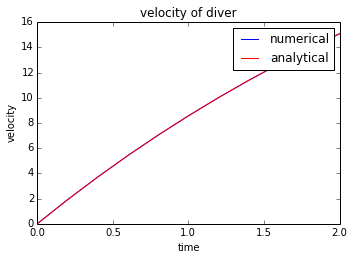
\includegraphics[max size={\textwidth}{\textheight}]{HW01_files/HW01_26_0.png}
    \par
    \end{center}
    
            \end{InvisibleVerbatim}
            
                \begin{InvisibleVerbatim}
                \vspace{-0.5\baselineskip}
    \begin{center}
    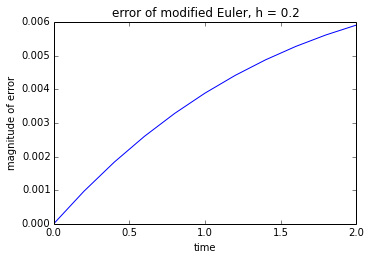
\includegraphics[max size={\textwidth}{\textheight}]{HW01_files/HW01_26_1.png}
    \par
    \end{center}
    
            \end{InvisibleVerbatim}
            
        
    

        

        \renewcommand{\indexname}{Index}
        \printindex

    % End of document
    \end{document}


